\documentclass[12pt]{article}

% Pretty much all of the ams maths packages
\usepackage{amsmath,amsthm,amssymb,amsfonts}

% Allows you to manipulate the page a bit
\usepackage[a4paper]{geometry}

% Pulls the page out a bit - makes it look better (in my opinion)
\usepackage{a4wide}

% Removes paragraph indentation (not needed most of the time now)
\usepackage{parskip}

% Allows inclusion of graphics easily and configurably
\usepackage{graphicx}

% Provides ways to make nice looking tables
\usepackage{booktabs}

% Allows you to rotate tables and figures
\usepackage{rotating}

% Allows shading of table cells
\usepackage{colortbl}
% Define a simple command to use at the start of a table row to make it have a shaded background
\newcommand{\gray}{\rowcolor[gray]{.9}}

\usepackage{textcomp}

% Provides commands to make subfigures (figures with (a), (b) and (c))
\usepackage{subfigure}

% Typesets URLs sensibly - with tt font, clickable in PDFs, and not breaking across lines
\usepackage{url}

% Makes references hyperlinks in PDF output
\usepackage{hyperref}

% Provides ways to include syntax-highlighted source code
\usepackage{listings}
\lstset{frame=single, basicstyle=\ttfamily}

% Provides Harvard-style referencing
\usepackage{natbib}
\bibpunct{(}{)}{;}{a}{,}{,}

% Provides good access to colours
\usepackage{color}
\usepackage{xcolor}

\usepackage{tikz}

% Simple command I defined to allow me to mark TODO items in red
\newcommand{\todo}[1] {\textbf{\textcolor{red}{#1}}}

% Allows fancy stuff in the page header
\usepackage{fancyhdr}
\pagestyle{fancy}

% Vastly improves the standard formatting of captions
\usepackage[margin=10pt,font=small,labelfont=bf, labelsep=endash]{caption}

% Standard title, author etc.
\title{Report: Super Vector Mario}
\author{by	Mikkel Bernt Buchvardt and Theodor Lars Nyholm Ommen}
\date{}
% Put text on the left-hand and right-hand side of the header
\fancyhead{}
\lhead{Super Vector Mario}
\rhead{Buchvardt - Ommen}
\chead{}

\usepackage{titletoc}

\renewcommand{\thepart}{\Alph{part}}

\renewcommand{\thesection}{\arabic{section}}
\renewcommand{\thesubsection}{\alph{subsection})}
\renewcommand{\thesubsubsection}{\alph{subsection}\alph{subsubsection})}

\titlecontents{chapter}
[2.65em]
{\addvspace{10pt}\bfseries}
{\contentslabel{2.3em}}
{\hspace*{-2.3em}}
{\space.\hfill\contentspage}


\definecolor{dkgreen}{rgb}{0,0.6,0}
\definecolor{gray}{rgb}{0.5,0.5,0.5}
\definecolor{mauve}{rgb}{0.58,0,0.82}

\lstset{frame=tb,
	language=Java,
	aboveskip=3mm,
	belowskip=3mm,
	showstringspaces=false,
	columns=flexible,
	basicstyle={\small\ttfamily},
	numbers=left,
	numberstyle=\tiny\color{gray},
	keywordstyle=\color{blue},
	commentstyle=\color{dkgreen},
	stringstyle=\color{mauve},
	breaklines=true,
	breakatwhitespace=true,
	tabsize=3
}






\begin{document}
  \maketitle

%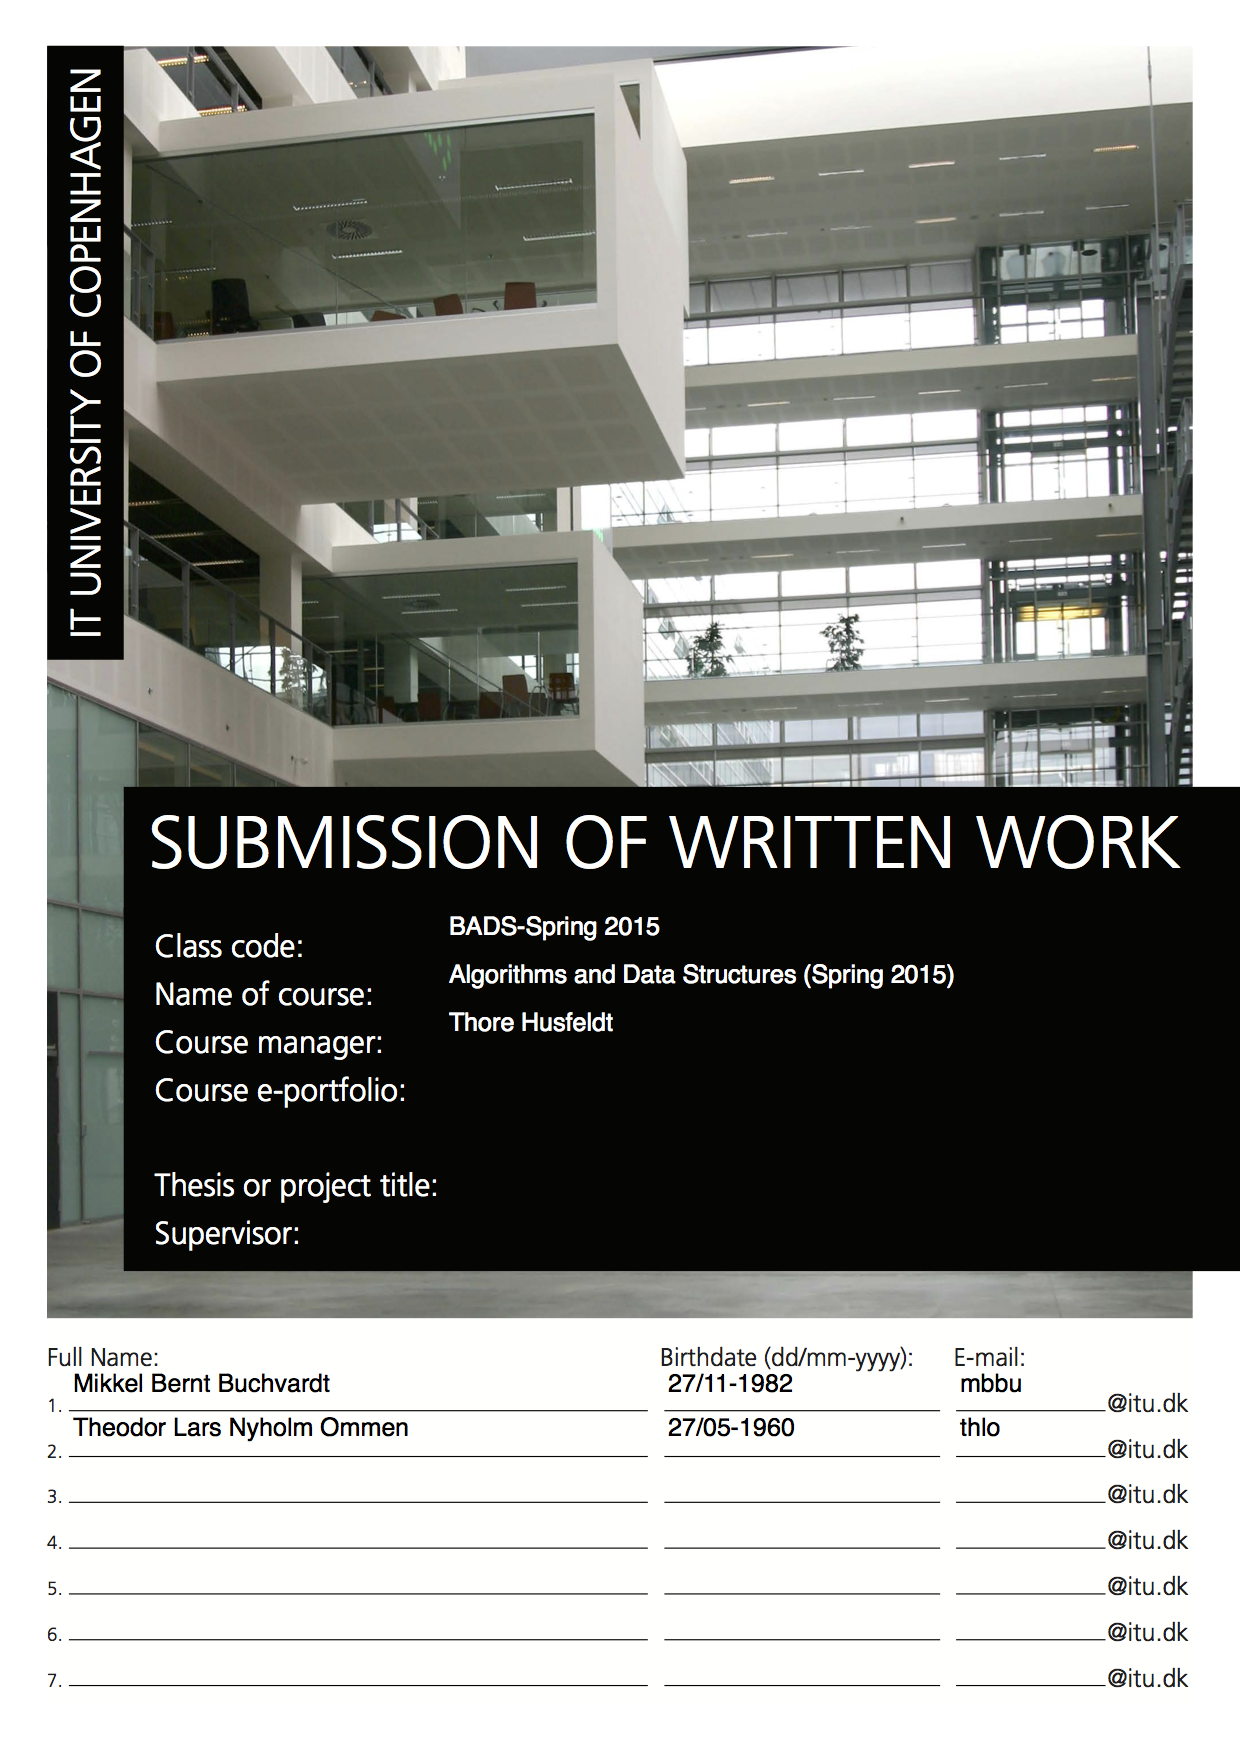
\includegraphics[scale=0.55]{frontpage}

  \section{Results}
  
  
  
  

  The following table summarizes our result:
  
    \bigskip\noindent
  \begin{tabular}{lr}
  	\toprule
  	Input file & MST total weight \\ \midrule
  	USA-highway-miles.txt	 & 16598.0 \\
  	tinyEWG-alpha.txt & 181 \\ \bottomrule
  \end{tabular}
  
    \bigskip
  
     The MST we found in tinyEWG-alpha.txt can be drawn like this:
     
     


  
  \section{Implementation details}
  
  We consider a map, where the coordinates come from loading the strings form the in-file into a String array.

  We talked about two ways to implement a solution:
  
  \begin{itemize}
  	\item starting in an S-field and pushing all legal fields from there to a queue and then pop the fields from the queue and push legal fields from these to the queue until a F-field is reached, counting each move and saving the smallest value for print in the end.
  	\item doing a recursive method that starts in a S-field and calls itself on all legal fields until a F-field is reached.
  	
 \end{itemize}	
 
 Pros and cons on each method made us decide on the first.
 
 The argument is as follows:
 
 If we store all visited fields with the speed we have visited them with in a simple table, we can check if we have been in a specific position with a specific speed (given by two coordinates) - if this is the case we do not go to this field again. This works because the algorithm gets us to a specific field in the shortes posible route.
 
 This is only true though if we use the queue method. Using the recursive method we might overshoot the target and get the first results of hitting an F on a longer route than the shortest (in fact this happens on all but the smallest maps). If we want to make the recursive method work we need to consider not only if we have been to a certain field with a certain speed but also if we have been there on a shorter route than the present.
 
 In other words the recursive method takes more calculations, more memory and more time.
  
  

\end{document}
